\section{Related Work}
%\subsection{Possible frameworks}
%There is a wide variety of web application frameworks. The PowerPedia prototype was build with the Recess PHP framework, but there are many %others, written in programming languages such as PHP, Ruby, Perl, or Java.  
%\subsection{Web platforms}
%\subsection{Energy feedback systems and community platforms} 
 
%- welche frameworks kommen in frage?
%- beispiele von web platformen, die diese framworks gebrauchen. 
%- wieso wurden diese frameworks gebraucht?

PowerPedia and the eMeter system combine different aspects such as web technologies and energy efficiency feedback, collaboration and energy conserving tips, as well as household-level and device-level feedback. For all those aspects, there exist numerous examples and related work.
First, I present collaborative platforms in general with their framework choices, then I give an overview over feedback devices, and last, I discuss systems that are similar to PowerPedia. 

\subsection{Collaborative web platforms}\label{sec:collaborative_web_platforms}
The role of the user in modern web application is quite different from the pre Web 2.0 \footnote{Web 2.0 is a term introduced by Tim O'Reilly to describe a new generation of web applications \cite{web2_0}} era. The web has become a collaborative medium, where users participate and collaborate to create content. Data is the driving force of web application.

There are many examples of web platforms that build on collaboration. One of the most prominent ones is certainly Wikipedia \footnote{\url{http://www.wikipedia.com}}, which only exists because of participating users. Wikipedia was launched in 2001 and consists of 19 millions articles, written by collaborators around the world \cite{wikipedia}. Users have the possibility to create new articles or edit existing articles by extending and changing them, making improvement suggestions, or uploading images and diagramms. Wikipedia is run on the MediaWiki wiki software application \footnote{\url{http://www.mediawiki.org}}. MediaWiki is written in PHP and was designed specifically for Wikipedia. 

Software development is another area where users typically collaborate. In projects where multiple developers work on the same code, a shared space for hosting and managing that code is needed. This is where hosting services such as Github \footnote{\url{https://github.com/}} come into play. Github offers accounts for open source projects and uses the Git \footnote{\url{http://git-scm.com/}} version control system. It also includes social media elements such as following other users or watch repositories. Since its launch in 2008, it has had more than one million commits and is becoming the most popular source code repository\cite{inquirer_github}.
Supposedly, Github is written using Ruby on Rails\footnote{Gibhub \url{http://rubyonrails.org/applications}}.

TODO: Another good example?

\subsection{Energy feedback systems}
Existing systems that provide feedback on the electricity usage generally try to help users better understand where energy is wasted and to form a basis for a conscious energy usage~\cite{mattern:inproc:2010}. Three different approaches for such tools can be distinguished. Household-level feedback systems  measure the consumption of the entire household. Devices of this category are mostly installed at the main energy line or in the fuse box. Feedback on a device-level is another approach. Those measuring tools are installed between the device's power plug and the power outlet and measure the consumption of the connected appliance. Lastly, systems can combine the two techniques and measure the energy consumption on household-level and device-level.

\subsubsection{Household level feedback}
\todo{extend section only if really relevant for this thesis}
Wattson\footnote{DIY Kyoto \url{http://www.diykyoto.com/}}, Onzo\footnote{Onzo \url{http://www.onzo.co.uk/}}, TED-1000\footnote{
TED-1000 \url{http://www.theenergydetective.com/}} or Current Cost\footnote{Current Cost \url{http://www.currentcost.com/}} are examples of commercially available solutions to measure the energy consumption on a household level.  Most of those systems have a display in one way or another that displays the current and historic consumption as well as monetary estimations.  

Wattson, for example, has tree components, a display, sensor clip and transmitter. The sensor clip is attached to wires running from the fuse box and the transmitter is installed near the electricity meter. Data collected by the sensor clip is transmitted wirelessly by the transmitter to the display. The display depicts the current electricity consumption in watts and the expected cost. The color of the display changes according to the energy usage in the household. 

As the above mentioned systems only measure the overall consumption, it is not possible to determine where exactly the energy is used. On the other hand, if energy conservation measures are applied, the resulting saving can be tracked quite as it is reflected in the decrease of the overall watt number.

\subsubsection{Device level feedback}
\todo{extend section only if really relevant for this work}
Device level feedback solutions provide more specific information on the energy consumption of individual appliances. Kill A Watt \footnote{Kill a Watt \url{http://www.p3international.com/products/special/P4400/P4400-CE.html}} and Click \footnote{Click \url{http://www.ewz.ch/}} are systems that use a small display to depict consumption data. Generally, the displayed information is of rather limited nature due to the size of the display.
 
By connecting devices to Kill A Watt, users can find out how efficient their appliances are. Its display shows the current consumption and the cumulative consumption in Kilowatt-hours (kWh). Electrical expenses can be calculated by different time periods up to a year. 

In contrast to Kill A Watt, solutions like Plogg \footnote{Plogg \url{http://www.plogginternational.com/}} and Energy UFO \footnote{UFO Power Center \url{http://www.energyufo.com/}} don't have a display. Both systems need external software to access measured data.
The Energy UFO interface is a simple application for the iPhone or iPad, data collected by Ploggs is transmitted to a host computer with the wireless ZigBee technology.  

All of the above mentioned products can only provide feedback on the devices that are directly attached to outlets. There is no possibility to determine the overall consumption of the household automatically. 
% In contrast to solutions
% Other work has been conducted
\subsubsection{Combined approaches}
In the work of Peterson et al.~\cite{Petersen_2009}, WattBot, a system to track real-time and historical home energy consumption is proposed.  
A data collection hub collects, stores and wirelessly broadcasts data from a circuit breaker box attached to the fuse box. The system breaks down the data collection by individual circuits, which makes it possible to determine the consumption of individual devices as long as they have their own circuit. The authors also propose a user interface for the iPhone and iPod touch. The interface shows a bar diagram of all circuits, sorted by usage. Each bar is colored according to the amount of electricity consumed (figure~\ref{wattbot}).

Other work has been conducted by Guinard et al.\cite{weiss:inprocMUM:2010}, which tries to overcome the drawbacks of socket monitoring systems. Each appliance is plugged into a Plogg meter and the system integrates the data from the various sensors nodes to provide both device-level and household-level feedback. A smart gateway discovers Ploggs by scanning the environment for Bluetooth devices in a regular interval. The gateway also includes a web server which exposes the Ploggs as RESTful resources. Data collected by the gateway is made available for users over a web and a mobile user interface. The user interfaces poll the gateway every few seconds to get real-time results.   	
In order to be able to determine the overall consumption, in this system and similar ones such as the commercially available AlertMe\footnote{AlertMe SmartEnergy \url{http://www.alertme.com/}}, every device needs to be connected to a sensor. This fact makes the installation expensive and cumbersome. 

\begin{figure}[htbp]
\begin{center}
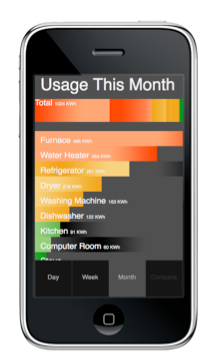
\includegraphics[width=4cm]{Images/wattbot.jpg}
\caption{Wattbot user interface}
\label{wattbot}
\end{center}
\end{figure} 
 

\subsection{Collaborative energy conservation platforms}
\subsubsection{Tips and ratings}
There exist various web platforms and sites to assist users in conserving energy. Especially websites with energy saving tips are quite numerous. Some of them encourage users to collaborate by offering the possibility to share their own energy saving ideas. The Swiss site of the World Wide Fund for Nature (WWF)~\cite{wwf} is a nice example. The focus is on using less resources in general, so electrical appliances are one of the main concerns, but not the only one. Users can rate tips and give feedback if they are already following the advice or if they are willing to do so in the future. Every tip displays the number of users who checked either of the two options as well as the average rating. At the same time, there is a mobile phone application that provides ratings on the efficiency of domestic appliances. Data is taken from the consumer webpage Topten.ch \footnote{\url{http://www.topten.ch/}}. Devices are sorted in device categories as found this website. For every category, the application lists the top products. On top of that, there are tips when buying a new device, device category specific tips to conserve energy, and further information such as existing labels, publications and links to external sources. So far, there is no user collaboration in the mobile phone app. Additionally, tips and further information are displayed in a text document fashion, which makes them tedious to read on a mobile phone. There is no "at one glance" overview and users have to do much scrolling to read the text.   

\subsubsection{Household level feedback}\label{sec:household_level_feedback}
For Wattson owners, there is the possibility of becoming a member of the Wattson community \footnote{\url{http://community.diykyoto.com/members}}. Registered users can download \textit{holmes}, a software that turns data collected by Wattson into plots and figures to illustrate the household energy usage. From \textit{holmes}, measurement data can be uploaded to the community portal. The portal is a means to display the overall energy (in kWh), power and CO2 (number of tonnes of carbon dioxide released into the atmosphere as a result of the electricity used). Users can chose a time period and one of the above options and the website displays the corresponding figure. Moreover, the amount of money spent on electricity is displayed on the page, although this feature is not quite clear as there is no further description (see figure~\ref{wattson_community}). According to the documentation, users should be able to compare their consumption to that of other users, but again, it is unclear how to do so on the page. At the time accessed\footnote{16.09.2011}, 2019 Wattson devices were connected to the portal. 
\begin{figure}[htbp]
\begin{center}
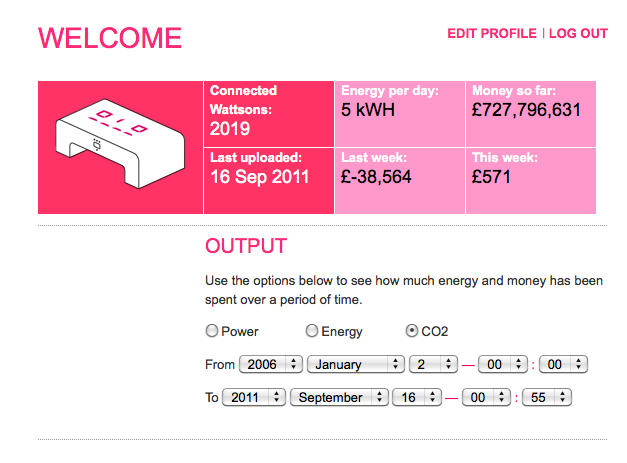
\includegraphics[width=12cm]{Images/wattson_community.png}
\caption{Wattson community portal}
\label{wattson_community}
\end{center}
\end{figure}

Another project, Velix \footnote{\url{http://velix.vkw.at}}, was developed by a group of researchers together with an Austrian electricity company \cite{energy_efficiency_online}. Velix provides users with feedback on their energy consumption and tips on how to save energy. The system aims at changing the users' behavior and daily routines. By giving them an overview over their energy consumption, users are supposed to get an idea of how much energy certain behaviors and routines need.  
Users are encouraged read their energy meter on a regular basis and publish the figures on the website on a weekly basis. Together with some general information about household size, heating method and house size, the energy efficiency of the user is calculated (see figure~\ref{velix}). 
In order to motivate a broader range of people to concern themselves with energy conservation, socio-psychological concepts were introduced in the project~\cite{improving_residential_energy_consumption}. Motivational elements such as rewards and commitment strategies help to keep users interested in the system. By uploading readings to Velix or fulfilling game-like tasks (such as signing up for a reminder to read the electricity meter, for example), points can be earned, which then can be exchanged for a real world gifts and prices.  
Velix was implemented with the open source content management system (CMS) Silverstripe \footnote{\url{http://www.silverstripe.com/}}.
\todo{what kind of feedback is given to users? Which paper is the theoretical basis for this project?}  
  
\begin{figure}[htbp]
\begin{center}
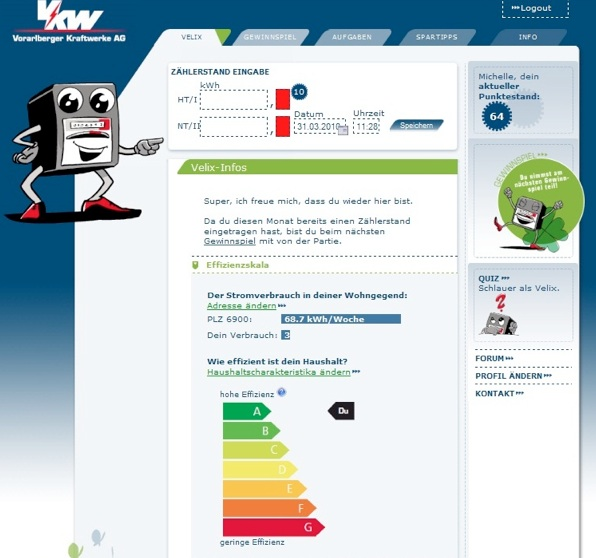
\includegraphics[width=12cm]{Images/velix.jpg}
\caption{Velix}
\label{velix}
\end{center}
\end{figure}  

People Power's Energy Services Platform\footnote{People Power Energy Services Platformhttp \url{http://peoplepowerco.com/mobile/}} has a slightly different approach. There is no designated web platform on its own, it is built as an iPhone and Android smartphone application and uses Facebook as a means to connect users. Also, there is no underlying sensing infrastructure, the application can be configured to work with one of two external products\footnote{Blue Line PowerCost Monitor \url{http://www.bluelineinnovations.com/} or TED 5000 \url{http://www.theenergydetective.com/}}. On top of being able to monitor, control and compare their total energy consumption, users can also compete against each others by completing a energy related quiz. The current score and rank can then be published on Facebook. Leaders and their high scores can be viewed at on the mobile phone application. The platform also has a Facebook page, where energy saving tips are published and users can comment on them\footnote{http://www.facebook.com/PeoplePowerCo}. 

%Users can monitor (current, historic or projected energy usage), control (set monthly budgets, get recommendations for energy efficient products), or compare (own, state and country's monthly average) their total energy consumption. Moreover, users can compete against each others by completing a energy related quiz. 

\subsubsection{Device level feedback}  
On device level, the Energy Literacy Platform  (ELP)\footnote{\url{http://www.sassor.com/}} is very promising project. Unfortunately, the platform is only a prototype. The platform was proposed by the Japanese start up Sassor in 2010 as a part of the E-idea Competition \footnote{\url{http://e-idea2010.climate-change.jp/en/}} by the British Councel \footnote{\url{http://www.britishcouncil.org/}}.
The proposed system consists of modules that can be plugged between the power plug and appliances, a receiver that collects the data from the different modules installed in the house, and the platform, which visualizes the measurements. The platform should display the consumption in real time (on both a device and household level), enable users to remotely switch on and off devices, compare values to friends and get energy saving tips.
Because there is no implementation yet, there are no further information on how data is compared, which framework and programming language is going to be used, or other details. 

\subsection*{Device comparison on consumer websites}
\todo{only to be included depending on focus of thesis}
Consumer webpages such as Sust-It\footnote{\url{http://www.sust-it.net}} or Topten\footnote{\url{http://www.topten.ch}} try to help users making more informed purchase decisions when it comes to energy efficiency. Both Sust-It and Topten use device categories and compare devices against devices in the same category. In order to make devices comparable, the criterion needs to be defined according to which devices are sorted. 

Sust-It ranks ranks devices according to their energy efficiency, which is expressed as the amount of energy devices use in one year (in Kilowatt-hours/year). In order to determine how many hours a device is in use per year, United Kingdom average values and other approximations are used. It is not further specified where the Kilowatt-hours value for a device is taken from.   

Topten uses a slightly different approach. Devices can be compared according to different criterions such as size, price, energy efficiency class or energy in kWh, just to name a few. Thus, there is no fixed ranking. According to their international website, in order to determine the energy efficiency of devices, "Topten relies on neutral tests and analysis of independent institutions, labels and on standardized declarations of manufacturers (e.g. EU-directives for household appliances)." \footnote{\url{http://www.topten.info/english/services/about_topten.html}}.